% Four-page topic proposal. Includes the empirical figure in ../figures/.
\documentclass[11pt,letterpaper]{article}
\usepackage[T1]{fontenc}
\usepackage[utf8]{inputenc}
\usepackage[margin=1in]{geometry}
\usepackage{lmodern,amsmath,amssymb,booktabs,enumitem,array,graphicx}
\usepackage{xcolor}
\definecolor{ink}{HTML}{223F91}
\usepackage[colorlinks=true,allcolors=ink]{hyperref}
\makeatletter
\renewcommand\section{\@startsection{section}{1}{\z@}{9pt}{4pt}{\normalfont\normalsize\bfseries\color{ink}}}
\makeatother
\setlength{\parindent}{0pt}
\setlength{\parskip}{4pt}
\setlist[itemize]{leftmargin=*,nosep,topsep=3pt}
\setlength{\abovedisplayskip}{6pt}
\setlength{\belowdisplayskip}{6pt}
\setlength{\abovedisplayshortskip}{4pt}
\setlength{\belowdisplayshortskip}{4pt}
\newcommand{\src}[2]{\hyperlink{ref:#1}{#2}}
\hypersetup{pdftitle={Economic freedom and firm entry--exit decisions},pdfauthor={Gabriel Saco}}

\begin{document}
{\Large\bfseries\color{ink} Economic freedom and firm entry--exit decisions}\par
\textbf{Gabriel Saco}\hfill Track B: model behind my thesis\par
\textit{Professor: Alexander Quispe}\hfill October 2026\par
\url{https://github.com/gsaco/ai-project}

\section{Question and track}
Why might an institutional deterioration cause a larger output loss than the
gain from an equal improvement? My thesis studies real GDP per capita after
economic-freedom changes (Figure~1). In this Track B project, I model a firm
that may close after a temporary setback. Even after institutions recover,
rebuilding may cost more than future earnings. The aim is to explain a possible
direction of asymmetry, rather than estimate the size of the GDP responses.

{\centering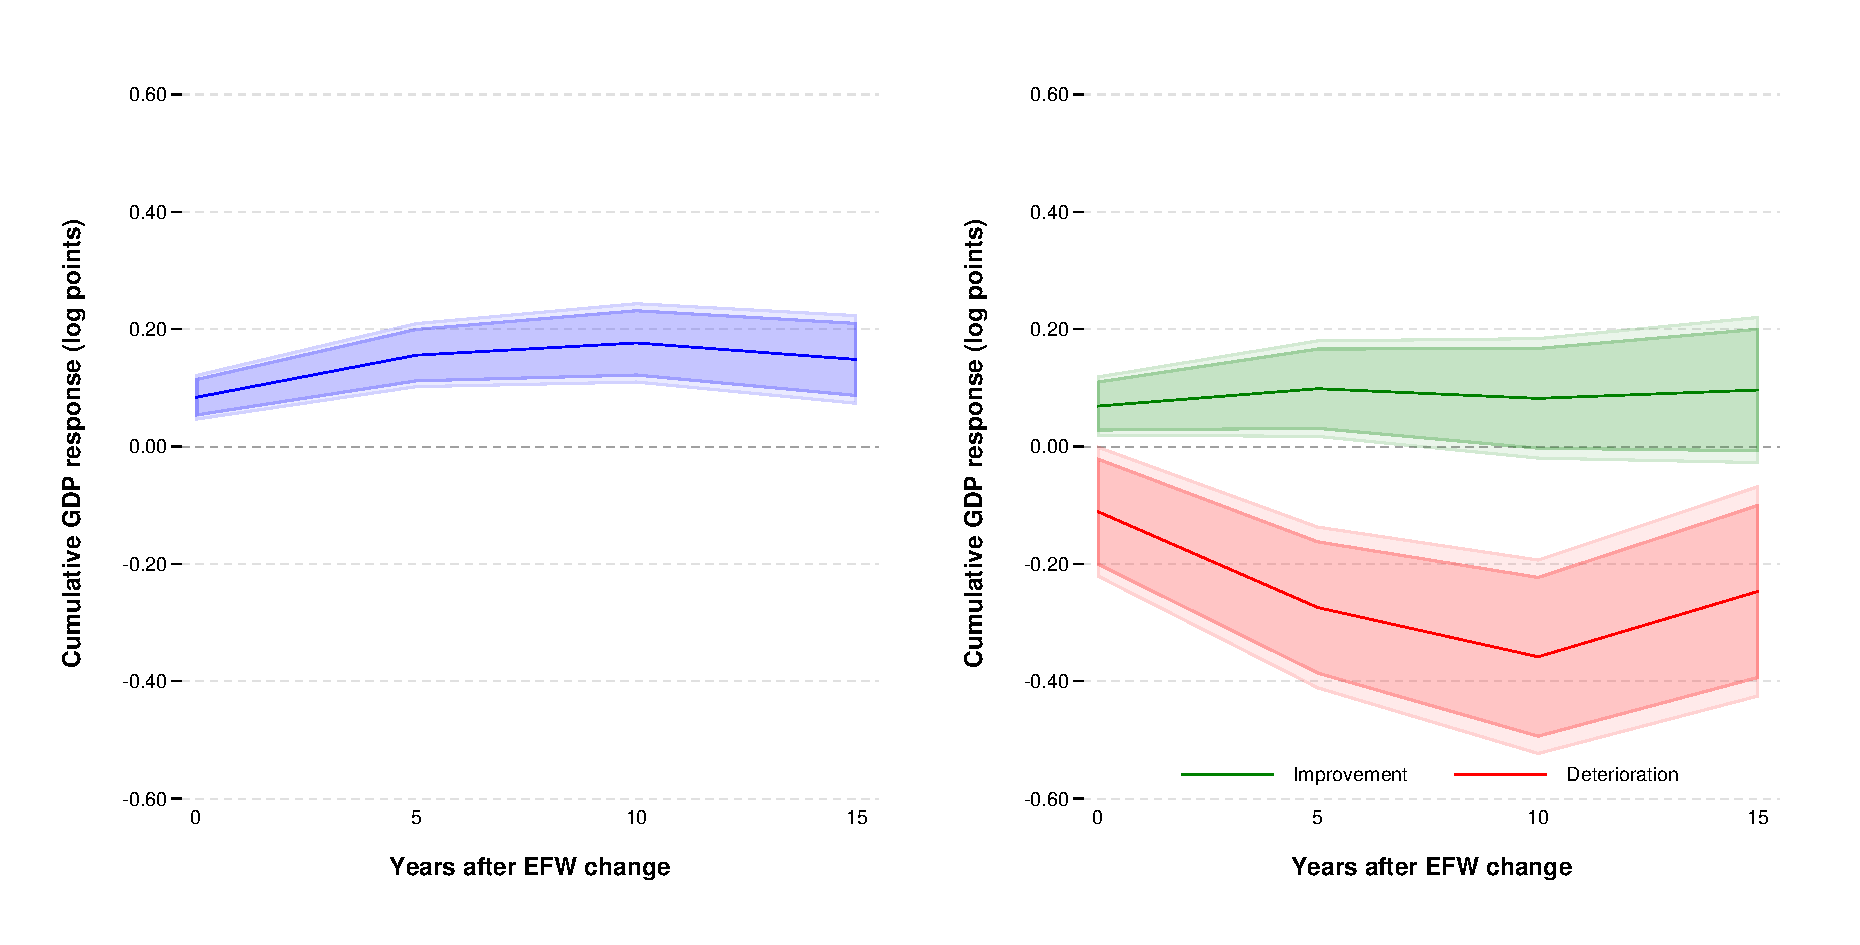
\includegraphics[width=0.68\linewidth]{../figures/paper_main_figure.pdf}\par}
{\footnotesize\textbf{Figure 1. Thesis evidence.} Cumulative log real GDP per capita
responses to one-point EFW changes, combining current and once-lagged effects.
Left: symmetry imposed; right: asymmetry allowed. Inner bands: 95\% country-clustered
pointwise intervals; outer: 95\% simultaneous sup-$t$ bands.\par}

\section{Baseline, changed assumption, and firm problem}\label{sec:setup}
\textbf{Baseline:} restarting is free, $\kappa=0$.
\textbf{Extension:} restarting requires a sunk cost, $\kappa>0$.
Technology, prices, other costs, and institutional paths are identical, isolating
the effect of restarting costs. The mechanism follows \src{dixit}{Dixit (1989)};
here the firm knows when institutions recover.

Economic freedom concerns property use, contracting, and exchange. The Economic
Freedom of the World (EFW) index measures government size, legal systems and
property rights, sound money, international trade, and regulation
\src{efw}{(Lawson et al., 2025)}. I summarize selected effects on firms through:
\begin{itemize}
\item $s\in(0,1]$ is the \textbf{institutionally usable share of fixed property}:
 title disputes or restrictions can make premises unavailable for production.
\item $c\geq0$ is \textbf{recurring institutional overhead}, paid while open
 independently of output, such as permit renewals or fixed reporting costs.
\end{itemize}
Several EFW areas may affect either channel. These firm conditions are not
index scores and do not cover every EFW component.

\textbf{Experiment.} The same firm starts open. Compare deterioration, no change,
and improvement: $s_0-d$, $s_0$, and $s_0+d$ at date~0, with $0<d<s_0$ and
$s_0+d\leq1$. All paths return permanently to $s_0$ from date~1, as known in
advance. Hold $c_t=c_0\geq0$ and all other parameters fixed.

\newpage
\textbf{Technology and choices.} The pre-existing property stock is $\bar k>0$;
usable property is $s\bar k$. With productivity $A>0$, elasticity $0<\alpha<1$,
and variable input $x\geq0$, assume Cobb--Douglas production. Choosing units
so that $\bar k=1$ gives
\begin{equation}\label{eq:technology}
q=A(s\bar k)^{1-\alpha}x^\alpha
\quad\xrightarrow{\bar k=1}\quad q=As^{1-\alpha}x^\alpha.
\end{equation}
For example, $s=0.5$ makes half the fixed stock usable. Output price is one;
input costs $w>0$ per unit. Operating overhead is $F+c_t$: ordinary fixed costs
$F>0$ plus institutional expenses $c_t\geq0$.

Activity is $a_t\in\{0,1\}$: open is one, closed is zero; initially $a_{-1}=1$.
Closure is free and preserves property but dismantles the organization. Opening
after closure costs $\kappa\geq0$. Financing is available, and no temporary
suspension option preserves the organization. The discount factor $0<\beta<1$
makes next period's unit of profit worth $\beta$ today. The firm solves
\begin{equation}\label{eq:problem}
\max_{\{a_t,x_t\}_{t\geq0}}\sum_{t=0}^{\infty}\beta^t
\left[As_t^{1-\alpha}x_t^\alpha-wx_t-(F+c_t)a_t
-\kappa a_t(1-a_{t-1})\right],
\end{equation}
subject to $x_t\geq0$ and $x_t=0$ if $a_t=0$. Each period contributes revenue
minus input spending, operating overhead, and any restart payment. The last
term charges $\kappa$ only when the firm moves from closed to open; earlier
setup costs have already been paid and cannot be recovered.

\section{Expected first-order condition and output responses}\label{sec:result}
\textbf{Step 1: choose input when open.} Today's input does not affect future
production opportunities or restart costs. Operating profit can therefore be
maximized separately in each period:
\begin{equation}\label{eq:static}
\pi(s,c)=\max_{x\geq0}\{As^{1-\alpha}x^\alpha-wx-F-c\}.
\end{equation}
Differentiating with respect to $x$ gives the first-order condition (FOC):
\begin{equation}\label{eq:foc}
\alpha As^{1-\alpha}x^{\alpha-1}-w=0
\quad\Longrightarrow\quad\boxed{\alpha As^{1-\alpha}x^{\alpha-1}=w.}
\end{equation}
Marginal revenue product equals input price. The second derivative is
$\alpha(\alpha-1)As^{1-\alpha}x^{\alpha-2}<0$; the slope falls from $+\infty$
to $-w$, giving a unique global optimum. Rearranging and substituting give
\begin{align}
 x^{1-\alpha}&=\frac{\alpha As^{1-\alpha}}{w}
 \quad\Longrightarrow\quad
 x^*(s)=s\left(\frac{\alpha A}{w}\right)^{1/(1-\alpha)},\label{eq:input}\\
 q(s)&=As^{1-\alpha}[x^*(s)]^\alpha
 =sA\left(\frac{\alpha A}{w}\right)^{\alpha/(1-\alpha)}.\label{eq:output}
\end{align}
Multiplying the FOC by $x^*$ yields $wx^*=\alpha q(s)$; therefore
\begin{equation}\label{eq:profit}
\pi(s,c)=q(s)-wx^*(s)-F-c=(1-\alpha)q(s)-F-c.
\end{equation}
Lower $s$ reduces optimal input, operating output, and profit; higher $c$ lowers
profit without changing input conditional on operating. Actual output is
$y_t=a_tq(s_t)$. \textbf{The FOC is unchanged across the baseline and extension:}
the restart cost does not depend on input use. The changed prediction concerns
activity and recovery, derived next.

\newpage
\textbf{Step 2: value operation and restarting.} Define normal output $q_0=q(s_0)$,
normal profit $\pi_0=\pi(s_0,c_0)>0$, and shock profits
$\pi_\pm=\pi(s_0\pm d,c_0)$. Equation~\eqref{eq:output} gives
\begin{equation}\label{eq:symmetry}
q(s_0\pm d)=q_0\left(1\pm\frac d{s_0}\right),
\qquad \pi_+-\pi_0=\pi_0-\pi_-.
\end{equation}
If the firm stays open, output and profit changes are equal and opposite.
Asymmetry therefore comes from closure. After restoration, an active firm
earns $\pi_0>0$ each period and has value
\begin{equation}\label{eq:value}
V=\pi_0+\beta\pi_0+\beta^2\pi_0+\cdots=\frac{\pi_0}{1-\beta}.
\end{equation}
A closed firm receives $V-\kappa$ from restarting or zero from staying out.
Waiting $n\geq0$ periods gives $\beta^n(V-\kappa)$: delay cannot improve on
immediate profitable restart or make a loss profitable. During the deterioration
at date~0, the firm compares
\begin{equation}\label{eq:closure}
\underbrace{\pi_-+\beta V}_{\text{continue}}
\qquad\text{and}\qquad
\underbrace{\beta\max\{V-\kappa,0\}}_{\text{close, retaining the restart option}}.
\end{equation}
A current loss alone need not cause closure: future profits can justify staying.

\textbf{Step 3: a conditional conjecture.} Keep all assumptions in
Section~\ref{sec:setup}, including available financing, no suspension that
preserves the organization, and the known institutional paths.
Assume
\begin{equation}\label{eq:conditions}
\boxed{\pi_0>0,\qquad\pi_-+\beta V<0,\qquad\kappa>\pi_++\beta V.}
\end{equation}
Then the firm closes at date~0 and never restarts after deterioration; it stays
open under no change or improvement. An otherwise identical inactive owner
facing the same setup cost stays out in every path.

\textbf{Argument.} Since $\pi_+>\pi_0$ and $\pi_0+\beta V=V$, the last inequality
implies $\kappa>V$, so closing is worth zero. Adverse continuation is negative;
normal and favorable continuation are positive. Favorable entry yields
$\pi_++\beta V-\kappa<0$; less profitable or delayed entry cannot do better.
The stronger cost bound excludes favorable entry; $\kappa>V$ alone suffices
for the incumbent's no-restart decision.

Let $y_t^-$, $y_t^0$, and $y_t^+$ denote output under deterioration, no change,
and improvement. Define the loss $L_t=y_t^0-y_t^-$ and gain $G_t=y_t^+-y_t^0$. Then
\begin{equation}\label{eq:dominance}
L_0=q_0>\frac d{s_0}q_0=G_0,\qquad
L_t=q_0>0=G_t\quad(t\geq1).
\end{equation}
The first inequality uses $d<s_0$. Closure removes all normal output; improvement
adds only a fraction. With \textbf{free restarting}, the same adverse firm closes
because $\pi_-<0$ but reopens at date~1 because $V>0$. With costly restarting
it remains closed: \textbf{full recovery becomes a persistent output shortfall}.
Impact asymmetry can occur in both cases; restarting costs change persistence.

A closed firm's log output is undefined. To compare positive totals, suppose
$Y_t^j=B+Ny_t^j$, where $B>0$ is unaffected output and $N>0$ is a fixed number
of identical firms. Hold $B$, $N$, and population fixed across paths. The
arithmetic--geometric mean inequality gives
\[
L_t\geq G_t\Rightarrow 2Y_t^0\geq Y_t^-+Y_t^+\geq2\sqrt{Y_t^-Y_t^+}
\Rightarrow \log Y_t^0-\log Y_t^-\geq\log Y_t^+-\log Y_t^0.
\]
This establishes a conditional positive-output comparison, not an estimated GDP effect.

\newpage
\section{Related literature and proposed contribution}
\src{dixit}{Dixit (1989)} explains why a firm's decision depends on whether
it already operates. A firm may tolerate losses to avoid rebuilding later;
once it closes, recovery may not justify restarting. His discussion of
organizational decay and temporary reversals (pp.~621, 623, 629) supplies the
mechanism used here. Persistence through sunk costs is an established result.

\src{dixit1992}{Dixit (1992, pp.~119--120)} distinguishes temporary suspension,
which can preserve the business, from abandonment, which may require rebuilding.
This identifies my model's main vulnerability: if waiting preserves the
organization cheaply, institutional recovery may also restore production.
The review includes this follow-up and its mathematical appendix.\footnote{The
earlier working paper and separate 1989 appendices were unavailable. The review
of Roberts and Tybout uses their published abstract.}

\src{dawson}{Dawson (1998)} connects institutions, investment, and growth.
At the firm level, \src{roberts}{Roberts and Tybout (1997)} report evidence of
sunk entry costs in Colombian export participation. This supports the relevance
of costly entry, without establishing the EFW--GDP mechanism studied here.

I apply the established restarting mechanism to known institutional changes.
The additional question is whether equal improvements and deteriorations
produce unequal output responses. Costly restarting alone does not guarantee
this direction. My contribution to the thesis is to state the conditions for
the comparison, derive it, and test how suspension or new entry changes it.
The proposal develops this application without claiming a new general theory.

\section{Plan and risks}
\textbf{Prove by hand.} I will show that the input choice is optimal, compare all
feasible sequences of opening and closing, and derive \eqref{eq:dominance} and
the log comparison for positive total output. The argument above is a proof outline;
a complete handwritten appendix remains future work.

\textbf{Simulate.} The current examples cover small shocks, free restarting,
and costly restarting. I will vary normal margins, shock size,
duration, and restart costs, and map continued operation, reopening, and permanent
closure. I will then examine overhead shocks, suspension, entry, and heterogeneity.
These are illustrative calculations, not empirical calibration.

\textbf{Formalize in Lean.} Lean will check that each conclusion follows from
its stated assumptions. I will begin with $(1-\beta)V=\pi_0$, the opening and
closing comparisons, and why delayed restarting cannot improve the firm's value.
I will then formalize optimal input and the output inequalities, using
AppliedModelingLib. This formal verification remains future work.

\textbf{Most likely failure.} A temporary setback may induce cheap suspension
without dismantling the organization. That option can remove the lasting loss;
it is the first robustness test. Entry and reallocation further challenge
aggregate persistence. Passing numerical checks will not replace a proof.

{\footnotesize\raggedright
\textbf{References}\par\setlength{\parskip}{2pt}
\hypertarget{ref:dixit}{}Dixit, A.~K. (1989).
\href{https://doi.org/10.1086/261619}{Entry and exit decisions under uncertainty}.
\emph{Journal of Political Economy}, 97(3), 620--638.\par
\hypertarget{ref:dixit1992}{}Dixit, A.~K. (1992).
\href{https://doi.org/10.1257/jep.6.1.107}{Investment and hysteresis}.
\emph{Journal of Economic Perspectives}, 6(1), 107--132.\par
\hypertarget{ref:roberts}{}Roberts, M.~J., and Tybout, J.~R. (1997).
\href{https://pure.psu.edu/en/publications/the-decision-to-export-in-colombia-an-empirical-model-of-entry-wi/}{The decision to export in Colombia: an empirical model of entry with sunk costs}.
\emph{American Economic Review}, 87(4), 545--564.\par
\hypertarget{ref:dawson}{}Dawson, J.~W. (1998).
\href{https://doi.org/10.1111/j.1465-7295.1998.tb01739.x}{Institutions, investment, and growth}.
\emph{Economic Inquiry}, 36(4), 603--619.\par
\hypertarget{ref:efw}{}Lawson, R., Murphy, R., and Mitchell, M.~D. (2025).
\href{https://www.cato.org/sites/cato.org/files/2025-09/economic-freedom-of-the-world-2025-chapter-1.pdf}{Economic freedom of the world in 2023}.
\emph{EFW: 2025 Annual Report}, ch.~1. Fraser Institute.
}
\end{document}
